% !TeX spellcheck = it_IT
\newpage
\section{Agenti risolutori di problemi}
Gli agenti risolutori di problemi adottano il paradigma della risoluzione di problemi come \textbf{ricerca} in uno \textbf{spazio di stati}. Sono agenti con \textbf{modello} (storia percezioni e stati) che adottano una rappresentazione \textbf{atomica} degli stati.\\
Sono particolari gli agenti con \textbf{obiettivo} che pianificano l'intera sequenza di mosse prima di agire.

\subsection{Processo di risoluzione}
I passi da seguire sono i seguenti:
\begin{enumerate}
	\item \textbf{Determinazione di un obiettivo}, ovvero un insieme di stati in cui l'obiettivo è soddisfatto
	\item \textbf{Formulazione} del problema tramite la rappresentazione degli stati e delle azioni
	\item Determinazione della \textbf{soluzione} mediante la ricerca
	\item \textbf{Esecuzione} del piano
\end{enumerate}

\begin{example}[Viaggio con mappa]
	Supponiamo di voler fare un viaggio. Il processo di risoluzione sarebbe il seguente:
	\begin{enumerate}
		\item Raggiungere Bucarest
		\item \begin{itemize}
			\item Azioni: guidare da una città all'altra
			\item Stato: città su mappa
		\end{itemize}
	\end{enumerate}
\end{example}

\subsection{Assunzioni}
Assumiamo che l'ambiente in questione sia \textbf{statico}, \textbf{osservabile}, \textbf{discreto} e \textbf{deterministico} (assumiamo un mondo ideale).

\subsection{Formulazione del problema}
Un problema può essere definito formalmente mediante 5 componenti:
\begin{enumerate}
	\item \textbf{Stato iniziale}
	\item \textbf{Azioni} possibili
	\item \textbf{Modello di transizione}: $ris: stato \times azione \to stato$, uno stato \emph{successore} $ris(s,a)=s'$
	\item \textbf{Test obiettivo} per capire tramite un insieme di stati obiettivo se il goal è raggiunto $test: stato \to \{true,false\}$
	\item \textbf{Costo del cammino}: composto dalla somma dei costi delle azioni, dove un passo ha costo $c(s,a,s')$. Un passo non ha mai costo negativo.
\end{enumerate}
I punti 1, 2 e 3 definiscono implicitamente lo \textbf{spazio degli stati}. Definirlo esplicitamente può essere molto costoso.

\subsection{Algoritmo di ricerca}
Gli algoritmi di ricerca prendono in input un problema e restituiscono un \textbf{cammino soluzione}.\\
Dobbiamo misurare le \textbf{prestazioni}: trova una soluzione? Quanto costa trovarla? Quanto è efficiente?
\begin{equation*}
	costo\_totale=costo\_ricerca+costo\_cammino\_sol
\end{equation*}

\begin{example}[Arrivare a Bucarest]
	Partiamo con la formulazione del problema:
	\begin{enumerate}
		\item \textbf{Stato iniziale}: la città di partenza, ovvero Arad
		\item \textbf{Azioni}: spostarsi in una città collegata vicina
		\begin{lstlisting}
			Azioni(In(Arad))={Go(Sibiu),Go(Zerind),...}
		\end{lstlisting}
		\item \textbf{Modello di transizione}: 
		\begin{lstlisting}
			Risultato(In(Arad), Go(Sibiu)) = In(Sibiu)
		\end{lstlisting}
		\item \textbf{Test obiettivo}:
		\begin{lstlisting}
			{In(Bucarest)}
		\end{lstlisting}
		\item \textbf{Costo del cammino}: somma delle lunghezze delle strade
	\end{enumerate}
	In questo esempio lo spazio degli stati coincide con la rete dei collegamenti tra le città.
	\begin{center}
		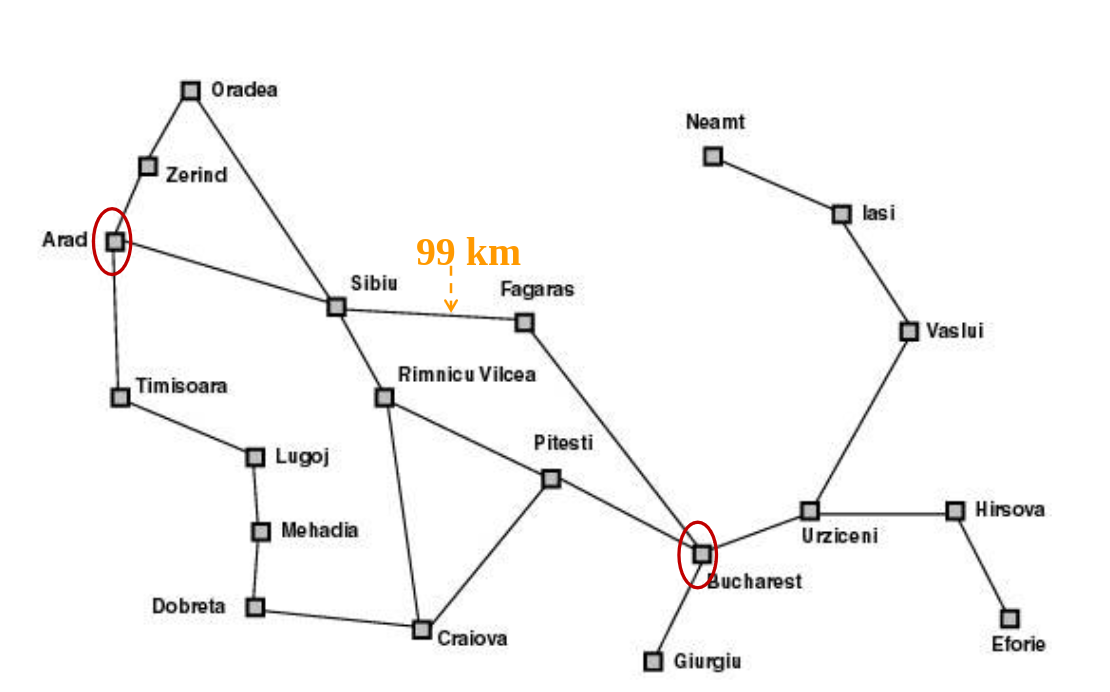
\includegraphics[scale=0.2]{bucarest_example.png}
	\end{center}
\end{example}

\begin{example}[Puzzle dell'8]
	Partiamo con la formulazione del problema:
	\begin{enumerate}
		\item \textbf{Stati}: tutte le possibili configurazioni della scacchiera
		\item \textbf{Stato iniziale}: una configurazione tra quelle possibili
		\item \textbf{Obiettivo}: una configurazione del tipo
		\begin{center}
			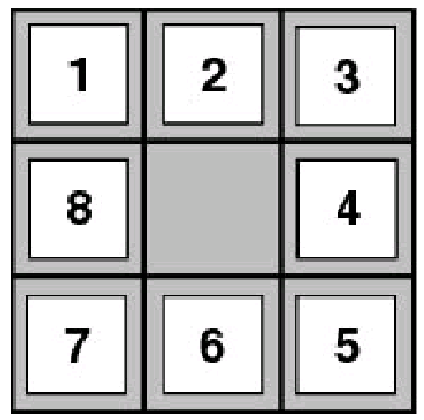
\includegraphics[scale=0.2]{8_puzzle_win.png}
		\end{center}
		\item \textbf{Azioni}: le mosse della casella vuota
		\item \textbf{Costo cammino}: ogni passo costa 1
	\end{enumerate}
	In questo esempio lo spazio degli stati è un grafo con possibili cicli (ci possiamo ritrovare in configurazioni già viste). Il problema è NP-completo: per 8 tasselli ci sono $\frac{9!}{2}=181.000$ stati.
\end{example}

\begin{example}[8 regine]
	Supponiamo di dover collocare 8 regine su una scacchiera in modo tale che nessuna regina sia attaccata da altre.
	\begin{enumerate}
		\item \textbf{Stati}: tutte le possibili configurazioni della scacchiera con 0-8 regine
		\item \textbf{Goal test}: avere 8 regine sulla scacchiera, di cui nessuna è attaccata
		\item \textbf{Azioni}: aggiungi una regina
	\end{enumerate}
	In questo esempio lo spazio degli stati sono le possibili scacchiere, ovvero $64 \times 63 \times \ldots \times 57 \simeq 1.8 \times 10^{14}$.\\
	Proviamo ad utilizzare una formulazione diversa:
	\begin{enumerate}
		\item \textbf{Stati}: tutte le possibili configurazioni della scacchiera in cui \emph{nessuna regina è minacciata}
		\item \textbf{Goal test}: avere 8 regine sulla scacchiera, di cui nessuna è attaccata
		\item \textbf{Azioni}: aggiungere una regina nella colonna vuota più a destra ancora libera in modo che non sia minacciata
	\end{enumerate}
	Lo spazio degli stati passa a $2057$, anche se comunque rimane esponenziale per $k$ regine.\\
	Vediamo infine un'ultima formulazione:
	\begin{enumerate}
		\item \textbf{Stati}: scacchiere con 8 regine, una per colonna
		\item \textbf{Goal test}: nessuna delle regine già presenti è attaccata
		\item \textbf{Azioni}: sposta una regina nella colonna se minacciata
		\item \textbf{Costo cammino}: zero
	\end{enumerate}
	Qui lo spazio degli stati è di qualche decina di milione.\\
	Capiamo quindi che formulazioni diverse del problema portano a spazi di stati di dimensioni diverse.
\end{example}

\begin{example}[Dimostrazione di teoremi]
	Dato un insieme di premesse:
	\begin{equation}
		\{s, t, q \Rightarrow p, r \Rightarrow p, v \Rightarrow q, t \Rightarrow r, s \Rightarrow v\}
	\end{equation}
	dimostrare una proposizione $p$ utilizzando solamente la regola di inferenza \emph{Modus Ponens}:
	\begin{equation*}
		(p \wedge p\Rightarrow q) \Rightarrow q
	\end{equation*}
	Scriviamo la formulazione del problema:
	\begin{itemize}
		\item \textbf{Stati}: insieme di proposizioni
		\item \textbf{Stato iniziale}: le premesse
		\item \textbf{Stato obiettivo}: un insieme di proposizioni contenente il teorema da dimostrare
		\item \textbf{Operatori}: l'applicazione del Modus Ponens
	\end{itemize}
	Lo spazio degli stati è quindi il seguente:
	\begin{center}
		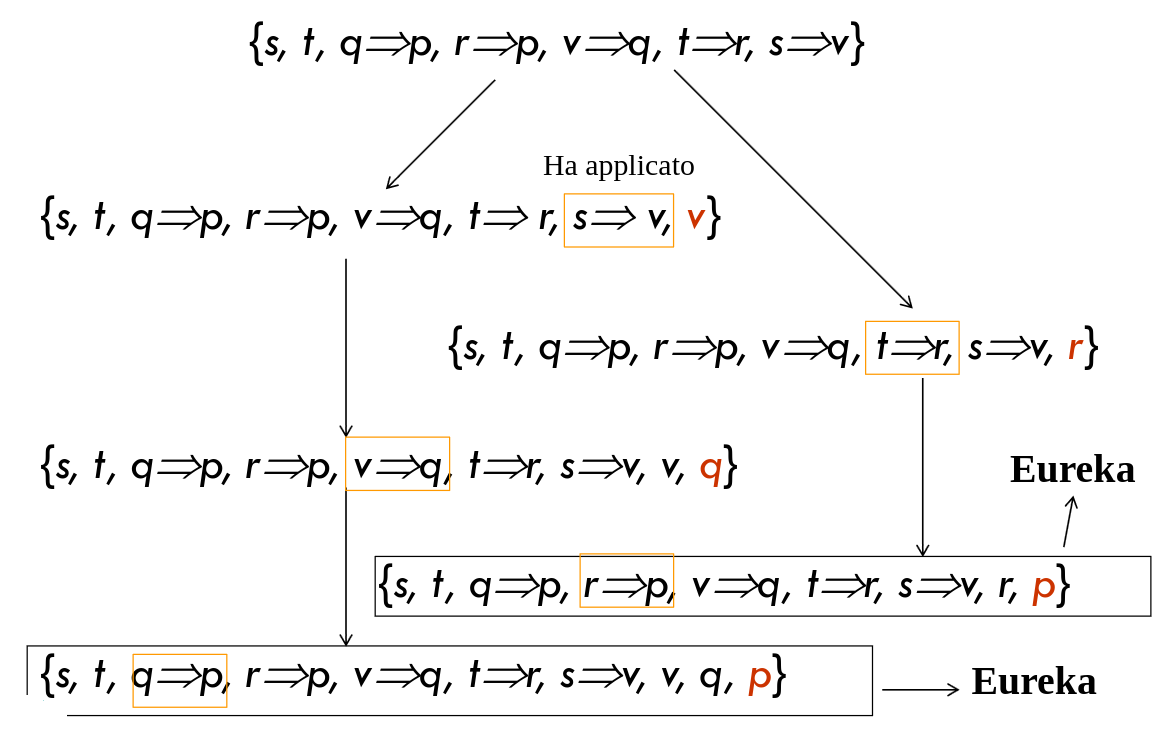
\includegraphics[scale=0.3]{dimostrazione_teoremi.png}
	\end{center}
\end{example}

%TODO Spostare da qui in poi in un altro file
\subsection{Ricerca della soluzione}
La ricerca della soluzione consiste nella generazione di un \textbf{albero di ricerca} a partire dalle possibili sequenze di azioni che si sovrappone allo spazio degli stati.\\
Ad esempio per il caso di Bucarest:
\begin{center}
	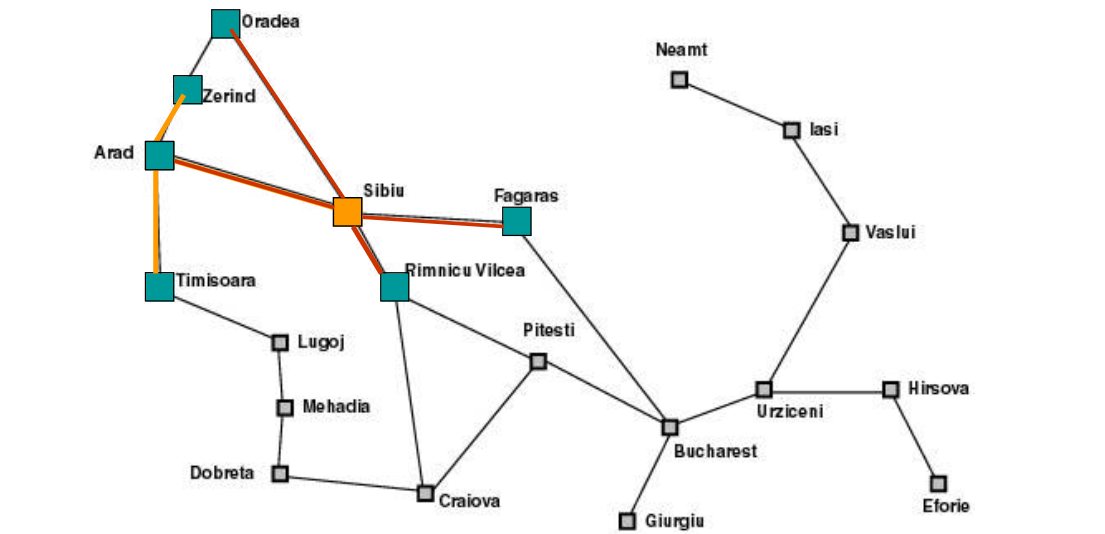
\includegraphics[scale=0.3]{bucarest_tree.png}
\end{center}
Espandiamo ogni nodo con i suoi possibili successori (frontiera).
\begin{definition}[Frontiera]
	Lista dei nodi in attesa di essere espansi (le foglie dell'albero di ricerca).
\end{definition}
\begin{observation}
	Si noti che un nodo dell'albero è diverso da uno stato. Infatti possono esitere nodi dell'albero di ricerca con lo stesso stato (si può tornare indietro).
\end{observation}

\subsection{Strategie di ricerca}
Ci sono diversi tipi di strategia per la ricerca della soluzione:
\begin{itemize}
	\item \textbf{FIFO}
	\item \textbf{LIFO}
	\item \textbf{Coda con priorità}
\end{itemize}

%TODO Ti sei perso delle slide

\subsubsection{Breadth First}
Come esplorare il grafo dello spazio degli stati a livelli progressivi di stessa profondità.\\
Per ogni nodo lo espandiamo, analizziamo i suoi figli (senza scendere ulteriormente di livello) e dopo averli fatti tutti scende di livello seguendo il principio FIFO.\\
Il seguente è il codice della \textbf{ricerca ad albero}, ovvero dove non si torna su un nodo già visitato.

\begin{lstlisting}
	function Ricerca-Ampiezza-A
		returns soluzione oppure fallimento
		nodo = un nodo con stato il problema.stato-iniziale e costo-di-cammino=0
		if problema.Test-Obiettivo(nodo.Stato) then return Soluzione(nodo)
		frontiera = una coda FIFO con nodo come unico elemento
	loop do
		if Vuota?(frontiera) then return fallimento
		nodo = POP(frontiera)
		for each azione in problema.Azioni(nodo.Stato) do
		figlio = Nodo-Figlio(problema, nodo, azione) [costruttore: vedi AIMA]
		if Problema.TestObiettivo(figlio.Stato) then return Soluzione(figlio)
		frontiera = Inserisci(figlio, frontiera) /* frontiera gestita come coda FIFO
	end
\end{lstlisting}

Il seguente è invece quello della \textbf{ricerca su grafo}:
\begin{lstlisting}
	function Ricerca-Ampiezza-g
		returns soluzione oppure fallimento
		nodo = un nodo con stato il problema.stato-iniziale e costo-di-cammino=0
		if problema.Test-Obiettivo(nodo.Stato) then return Soluzione(nodo)
		frontiera = una coda FIFO con nodo come unico elemento
		esplorati = insieme vuoto
	loop do
		if Vuota?(frontiera) then return fallimento
		nodo = POP(frontiera); aggiungi nodo.Stato a esplorati
		for each azione in problema.Azioni(nodo.Stato) do
		figlio = Nodo-Figlio(problema, nodo, azione)
		if figlio.Stato non e in esplorati e non in frontiera then
		if Problema.TestObiettivo(figlio.Stato) then return Soluzione(figlio)
		frontiera = Inserisci(figlio, frontiera) /* in coda
	end
\end{lstlisting}

\noindent Analizziamone la complessità partendo dalle seguenti assunzioni:
\begin{itemize}
	\item Fattore di \textbf{branching} $b$: numero massimo di successori
	\item \textbf{Depth} del nodo obiettivo più superficiale
	\item Lunghezza \textbf{massima} dei cammini nello spazio degli stati
\end{itemize}
La strategia è ottimale se tutti gli operatori hanno lo stesso costo $k$, ovvero se $g(n)=k \cdot depth(n)$, dove $g(n)$ è il costo del cammino per arrivare ad $n$.\\
La complessità nel \emph{tempo} (nodi generati) sarà 
\begin{equation*}
	T(b,d)=1+b+b^2+\ldots+b^d \longrightarrow O(b^d)
\end{equation*}
mentre in \emph{spazio} (nodi in memoria):
\begin{equation*}
	O(b^d)
\end{equation*}
È chiaro che l'algoritmo scali male, sopratutto per quanto riguarda lo spazio.

\subsubsection{Depth first}
In questo algoritmo si parte da un nodo e si scende nel primo figlio, procedendo appunto in profondità. Arrivati alle foglie si torna indietro ai figli precedentemente non visitati. In memoria tengo solamente  i fratelli del path corrente ed elimino i rami già esplorati.\\  Possono esserci tre versioni possibili:
\begin{itemize}
	\item \textbf{Albero}: data $m$ la lunghezza massima dei cammini nello spazio degli stati e $b$ il fattore di diramazione, la \textbf{complessità} in \emph{tempo} è $O(b^m)$ (può essere maggiore di $O(b^d)$) mentre in \emph{spazio} è $b \cdot m$.
	Rispetto al Breadth First, non è né completo né ottimale, ma ci garantisce un notevole risparmio in memoria
	\item \textbf{Grafo}: la memoria corrisponde a tutti i possibili stati, diventando quindi completo nello spazio finito (non in quello infinito)
	\item \textbf{Ricorsiva}: ancora più efficiente per la memoria perché mantiene solo il cammino corrente ($O(m)$). Viene realizzata con un algoritmo di \emph{backtracing} che salva lo stato su uno stack a cui torna in caso di fallimento.
\end{itemize}
\newpage
\begin{lstlisting}
	function Ricerca-DF-A (problema)
		returns soluzione oppure fallimento
		return Ricerca-DF-ricorsiva(CreaNodo(problema.Stato-iniziale), problema)
	
	function Ricerca-DF-ricorsiva(nodo, problema)
		returns soluzione oppure fallimento
		if problema.TestObiettivo(nodo.Stato) then return Soluzione(nodo)
		else
		for each azione in problema.Azioni(nodo.Stato) do
			figlio = Nodo-Figlio(problema, nodo, azione)
			risultato = Ricerca-DF-ricorsiva(figlio, problema)
			if risultato != fallimento then return risultato
		return fallimento
\end{lstlisting}
\subsubsection{Depth Limited}
La ricerca in profondità limitata arriva fino ad un dato livello $l$. È completa solo se si conosce il limite superiore $d$ per la profondità della soluzione e $d<l$. Non è ottimale e ha complessità in tempo $O(b^l)$ e in spazio $O(b \cdot l)$
\subsubsection{Iterative Depth}
Questo approccio prevede di provare l'algoritmo depth limited con limite di profondità $l=0, 1, \ldots$ fino a trovare la soluzione. È il miglior compromesso tra breadth first e depth first:
\begin{itemize}
	\item Complessità in \textbf{tempo} $O(b^d)$ se ammette soluzione
	\item Complessità in \textbf{spazio} $O(b \cdot d)$ se ammette soluzione
\end{itemize}
Quindi ha la \emph{completezza} e l'\emph{ottimalità} del breadth first e la complessità in \emph{spazio} della depth first.
\subsubsection{Uniform Cost}
Partendo da una ricerca in ampiezza, la generalizziamo: si sceglie il nodo di costo minore sulla frontiera e si espande sui contorni di costo uguale.
\begin{center}
	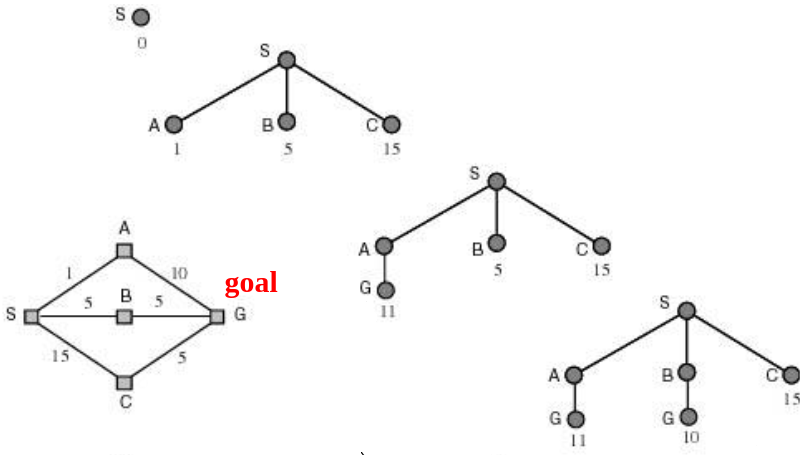
\includegraphics[scale=0.4]{uc.png}
\end{center}
\newpage
Codice per la ricerca su albero:
\begin{lstlisting}
	function Ricerca-UC-A (problema)
			returns soluzione oppure fallimento
			nodo = un nodo con stato il problema.stato-iniziale e costo-di-cammino=0
			frontiera = una coda con priorita con nodo come unico elemento
		loop do
			if Vuota?(frontiera) then return fallimento
			nodo = POP(frontiera)
			if problema.TestObiettivo(nodo.Stato) then return Soluzione(nodo)
			for each azione in problema.Azioni(nodo.Stato) do
				figlio = Nodo-Figlio(problema, nodo, azione)
				frontiera = Inserisci(figlio, frontiera) /* in coda con priorita*/
	end
\end{lstlisting}
Codice per la ricerca su grafo:
\begin{lstlisting}
	function Ricerca-UC-G (problema)
			returns soluzione oppure fallimento
			nodo = un nodo con stato il problema.stato-iniziale e costo-di-cammino=0
			frontiera = una coda con priorita con nodo come unico elemento
			esplorati = insieme vuoto
		loop do
			if Vuota?(frontiera) then return fallimento
			nodo = POP(frontiera);
			if problema.TestObiettivo(nodo.Stato) then return Soluzione(nodo)
			aggiungi nodo.Stato a esplorati
			for each azione in problema.Azioni(nodo.Stato) do
				figlio = Nodo-Figlio(problema, nodo, azione)
				if figlio.Stato non in esplorati e non in frontiera then
					frontiera = Inserisci(figlio, frontiera) /* in coda con priorita
				else if figlio.Stato in frontiera con Costo-cammino piu alto then
					sostituisci quel nodo frontiera con figlio */
	end
\end{lstlisting}
Questo algoritmo è \textbf{ottimo} e \textbf{completo} purché il costo degli archi sia $\epsilon > 0$. Assunto $C^*$ come costo della soluzione ottima, $\lfloor \frac{C^*}{\epsilon}\rfloor$ è il numero di mosse nel caso peggiore. La complessità è quindi $O(b^{1+\lfloor \frac{C^*}{\epsilon}\rfloor})$.
\begin{note}
	Quando ogni azione ha lo stesso costo, la complessità si avvicina a quella della breadth first: $O(b^{1+d})$.
\end{note}
\subsection{Direzione}
Un problema importante è quello della \textbf{direzione} della ricerca, che può essere:
\begin{itemize}
	\item In \textbf{avanti} o guidata da \emph{dati}: si esplora lo spazio di ricerca dallo stato iniziale all'obiettivo
	\item All'\textbf{indietro} o guidata dall'\emph{obiettivo}: si esplora lo spazio di ricerca partendo da uno stato goal e riconducendosi ad un sotto-goal fino a trovare uno stato iniziale
\end{itemize}
Per scegliere la direzione bisogna tenere in conto di quale ha il \textbf{fattore di diramazione} minore.  Si preferisce la ricerca all'\emph{indietro} quando l'obiettivo è ben definito (e.g. theorem proving) mentre quella in \emph{avanti} quando ci sono molteplici obiettivi (e.g. design).\\
\subsubsection{Ricerca bidirezionale}
Nella ricerca bidirezionale si procede in entrambe le direzioni fino ad incontrarsi. La \textbf{complessità} è:
\begin{itemize}
	\item \emph{Tempo}: $O(\sqrt{b^d})$ assumendo che il test dell'intersezione delle due direzioni sia costante
	\item \emph{Spazio}: $O(\sqrt{b^d})$, poiché almeno tutti i nodi di una direzione saranno in memoria
\end{itemize}
Si noti che non sempre è applicabile, come nel caso in cui i predecessori non siano definiti o ci siano troppi stati obiettivo.

\subsection{Problematiche}
\subsubsection{Cicli}
I cammini ciclici rendono gli alberi di ricerca \emph{infiniti} anche quando lo spazio degli stati è finito.
\begin{center}
	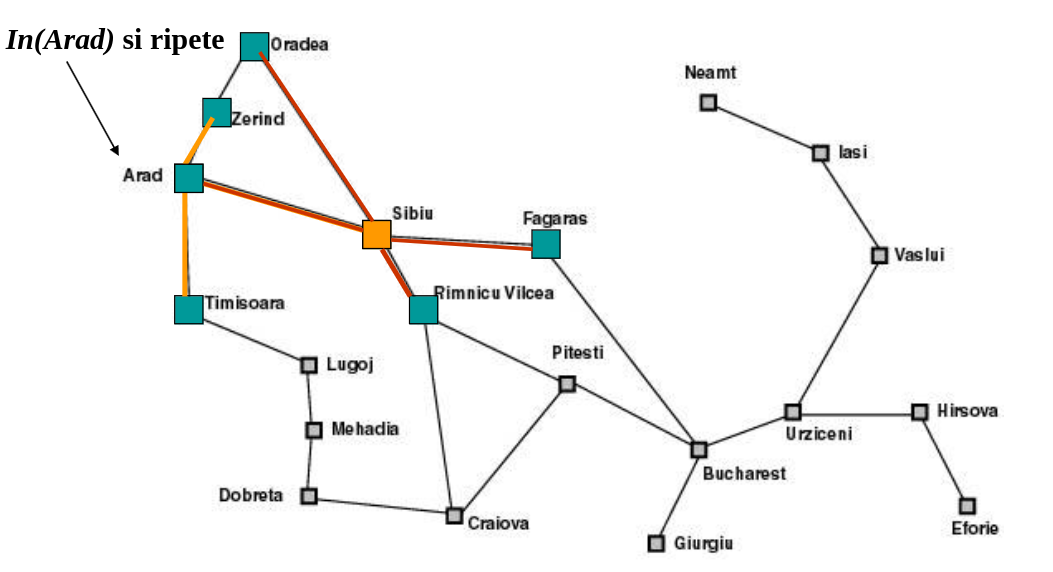
\includegraphics[scale=0.4]{cicli.png}
\end{center}
\subsubsection{Ridondanze}
Su spazi di stati a grafo si possono generare più volte nodi con lo stesso stato nella ricerca, anche in assenza di cicli.
\begin{center}
	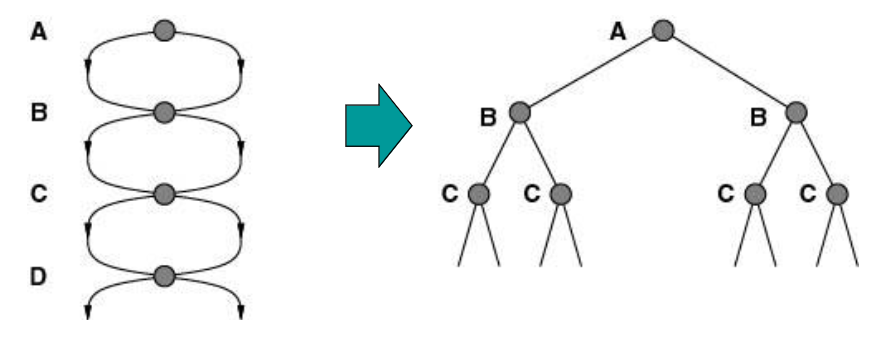
\includegraphics[scale=0.4]{ridondanze.png}
\end{center}
Visitare questi stati è lavoro inutile. Per evitarlo serve \textbf{ricordare} gli stati già visitati, occupando ovviamente più spazio. Tre possibili soluzioni sono:
\begin{enumerate}
	\item Non tornare nel nodo \textbf{genitore}, eliminandolo dai successori (non evita i cammini ridondanti)
	\item Per evitare i \textbf{cammini ciclici} si controlla che  i successori non siano antenati del nodo corrente
	\item Non generare nodi con \textbf{stati già esplorati}: ogni nodo visitato deve essere salvato in memoria
\end{enumerate}
Il costo può essere alto, ad esempio nella depth first la complessità in spazio torna ad essere pari a tutti gli stati.\\
La \textbf{ricerca} sul grafo avverrà quindi come segue:
\begin{enumerate}
	\item Mantiene una lista di stati esplorati (lista chiusa)
	\item Prima di espandere un nodo si controlla se era già stato incontrato o se è già nella frontiera
	\item In quel caso, non viene espanso
\end{enumerate}
Questa tecnica è ottimale solo se abbiamo la garanzia che il costo del nuovo cammino sia maggiore o uguale, ovvero non convenga.
\subsection{Confronto}
\begin{table}[!h]
	\centering
	\begin{tabular}{|c|c|c|c|c|c|c|}
		\hline
		\textbf{Confronto} & \textbf{BF} & \textbf{UC} & \textbf{DF} & \textbf{DL} & \textbf{ID} & \textbf{BDir}\\
		\hline
		Completa & Si & Si(*) & No & Si(**) & Si & Si(***)\\
		Tempo &$O(b^d)$ &$O(b^{1+\lfloor \frac{C^*}{\epsilon}\rfloor})$ & $O(b^m)$ & $O(b^l)$ & $O(b^d)$ & $O(\sqrt{b^d})$ \\
		Spazio &$O(b^d)$ &$O(b^{1+\lfloor \frac{C^*}{\epsilon}\rfloor})$ & $O(b\cdot m)$ & $O(b\cdot l)$ & $O(b\cdot d)$ & $O(\sqrt{b^d})$\\
		Ottimale & Si(****) & Si(*)& No & No & Si(****)& Si(***)\\
		\hline
	\end{tabular}
\end{table}
Legenda:
\begin{itemize}
	\item  \textbf{*}: se $\text{costo archi} \geq \epsilon \geq 0$
	\item \textbf{**}:  se si conosce il limite alla profondità della soluzione ($l>d$)
	\item \textbf{***}: se si utilizza UC o BF
	\item \textbf{****}: se gli archi hanno tutti lo stesso costo
\end{itemize}
